\section{Thu thập phân cụm người dùng từ Career Interest Clustering} \label{3.3}
Sử dụng bộ khung 16 ô được Phòng Công nghệ và Giáo dục Oklahoma xây dựng để xác định nhóm ngành phù hợp của người dùng, cũng là để trả lời cho câu hỏi ``Điều gì bạn giỏi?" (What are you good at?). Khảo sát bao gồm 16 khung như hình dưới đây:

\begin{figure}[H]
    \centering
    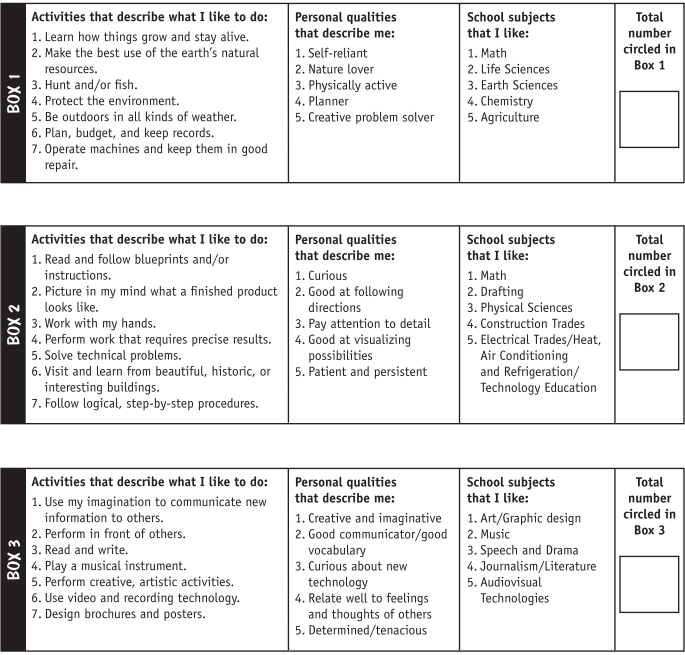
\includegraphics[width=0.9\linewidth]{images/chap3/CC1.png}
\end{figure}

\begin{figure}[H]
    \centering
    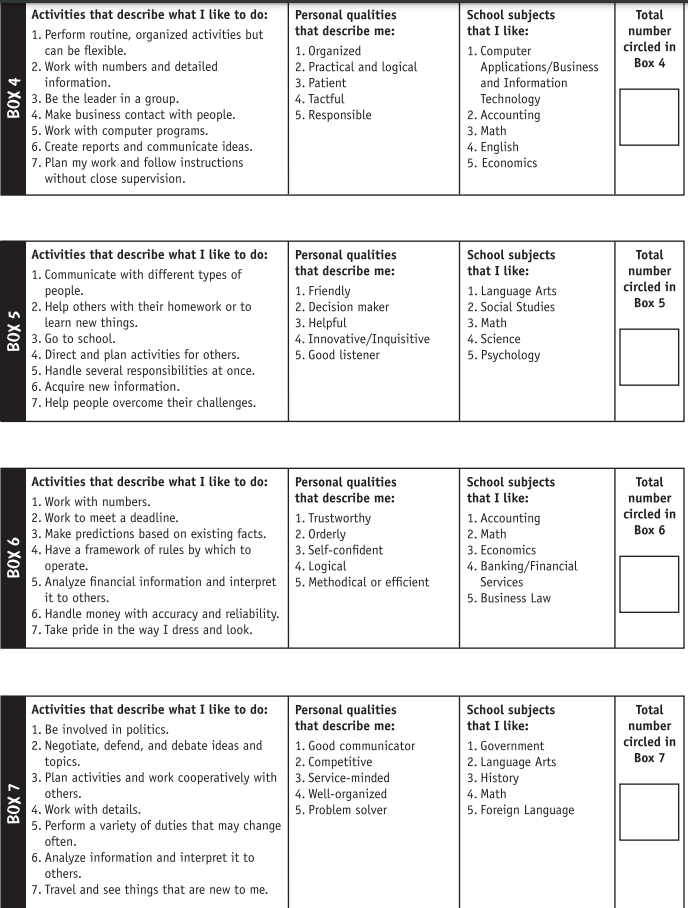
\includegraphics[width=0.9\linewidth]{images/chap3/CC2.png}
\end{figure}

\begin{figure}[H]
    \centering
    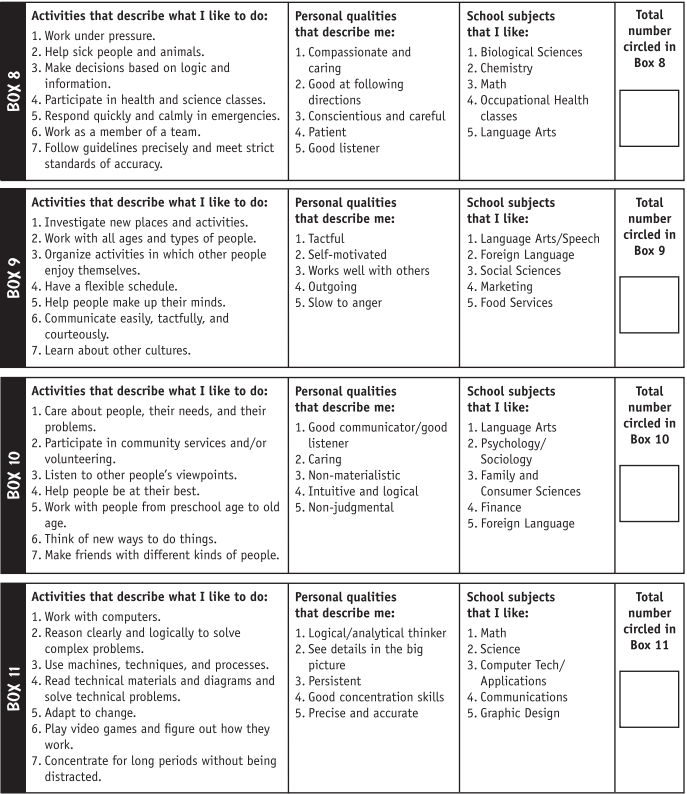
\includegraphics[width=0.9\linewidth]{images/chap3/CC3.png}
\end{figure}

\begin{figure}[H]
    \centering
    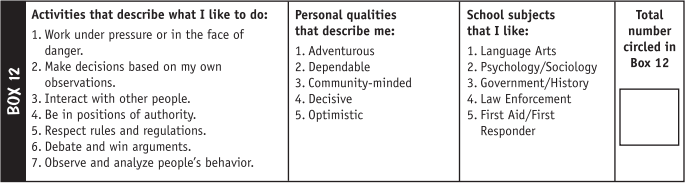
\includegraphics[width=0.9\linewidth]{images/chap3/CC4.png}
\end{figure}

\begin{figure}[H]
    \centering
    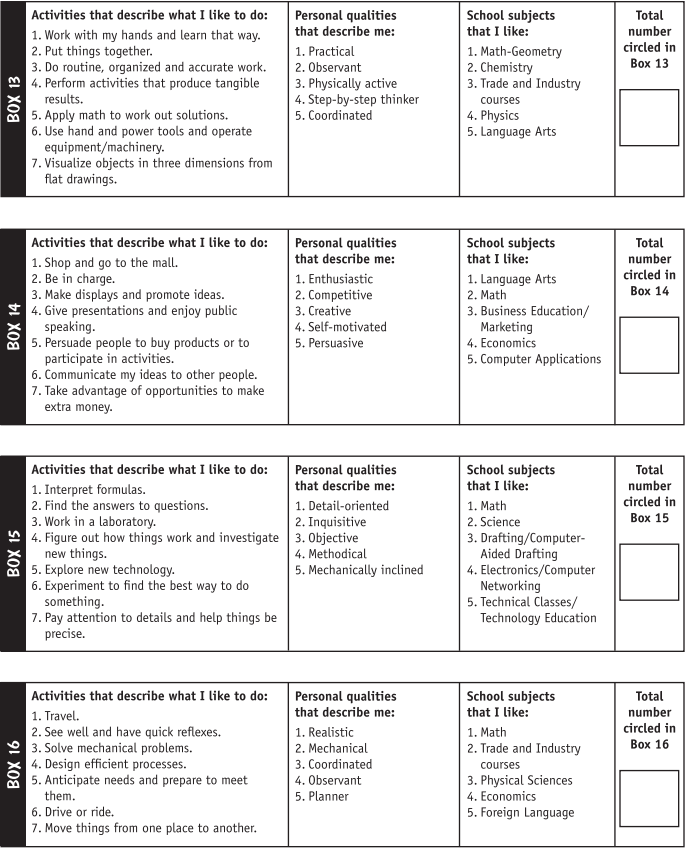
\includegraphics[width=0.9\linewidth]{images/chap3/CC5.png}
\end{figure}

Sau khi người dùng chọn những ô mà mình cảm thấy phù hợp trong mỗi box, box có điểm cao nhất sẽ tương ứng với ngành phù hợp cho người dùng trong career clustering, bao gồm theo các thứ tự đã được đề cập ở \hyperref[2.1.3]{phần 2.1.3}, từ đó có thể xác định được ngành phù hợp với mình, cũng như trả lời cho câu hỏi Điều gì bạn thật sự giỏi và làm tốt.